\begin{figure}[H]
\centering
\includegraphics[page=6,width=0.4\textwidth]{\FCNCFigures/tthML/showFake/faketau/postfit/NOMINAL/reg1l1tau1b3j_os_vetobtagwp70_highmet/chi2.pdf}
\put(-50, 80){\textbf{(a)}}
\put(-57, 95){\footnotesize{STH $\tlhad$}}
\includegraphics[page=6,width=0.4\textwidth]{\FCNCFigures/tthML/showFake/faketau/postfit/NOMINAL/reg1l1tau1b2j_os_vetobtagwp70_highmet/chi2.pdf}
\put(-50, 80){\textbf{(b)}}
\put(-57, 95){\footnotesize{TTH $\tlhad$}}\\
\includegraphics[page=6,width=0.4\textwidth]{\FCNCFigures/xTFW/showFake/NOMINAL/reg2mtau1b3jos_vetobtagwp70_highmet/chi2.pdf}
\put(-50, 80){\textbf{(c)}}
\put(-57, 95){\footnotesize{STH $\thadhad$}}
\includegraphics[page=6,width=0.4\textwidth]{\FCNCFigures/xTFW/showFake/NOMINAL/reg2mtau1b2jos_vetobtagwp70_highmet/chi2.pdf}
\put(-50, 80){\textbf{(d)}}
\put(-57, 95){\footnotesize{TTH $\thadhad$}}
\caption{ The distributions of $\chi^2$ in Eq. \ref{eq:eq2} in the hadronic channels. }
\label{fig:chi2}
\end{figure}
